%!TEX root = main.tex
\section{Modelling}
This report seeks to model the time evolution of a virus outbreak on earth. To do, firstly it will be described how one might model a virus outbreak in small uniform population. Secondly, this model will be expanded to include multiple population groups and their interactions. 

\subsection{The SIR Model}
\todo{cite stuff in this section}
\subsubsection{Assumption}
The Susceptible-Infected-Removed model is compartmental model assuming that within some subdivision of the population containing $N$ individuals, virus infection, cure and spread rates are i.i.d. for the 3 "compartments" of individuals:
\begin{itemize}
	\item Susceptible to the virus
	\item Infected by the virus
	\item Recovered and immune to the virus (or alternatively dead)
\end{itemize} 
. In reality economic status, job type, air-conditioning etc. will affect how a virus spread, however, depending on the heterogeneity of the population these assumptions constitute a good approximation. 

\subsubsection{Governing equations}
The SIR model is governed by 3 differential equations,
\begin{align}
\frac{d S(t)}{dt} &= - \frac{\beta}{N} I(t) S(t)   \label{eq-S}\\
\frac{d I(t)}{dt} &= \frac{\beta}{N} I(t) S(t) - \gamma I(t)  \label{eq-I}\\
\frac{d R(t)}{dt} &= \gamma I(t) \label{eq-R}
\end{align}
where $S(t), I(t)$ and $R(t)$ are functions describing the number of susceptible, infected and removed individuals at time t, $\beta$ is the rate of infection, $\gamma$ the rate of cure and $N$ the total number of individuals.

From equation \eqref{eq-S} and one \eqref{eq-I} can see that susceptible individuals become infected by some ratio proportional to $\beta$ and the ratio of already infected/susceptible individuals. From \eqref{eq-I} and \eqref{eq-R} one can see that infected individuals recover with a constant time factor. 

\begin{figure}[H]
	\centering
	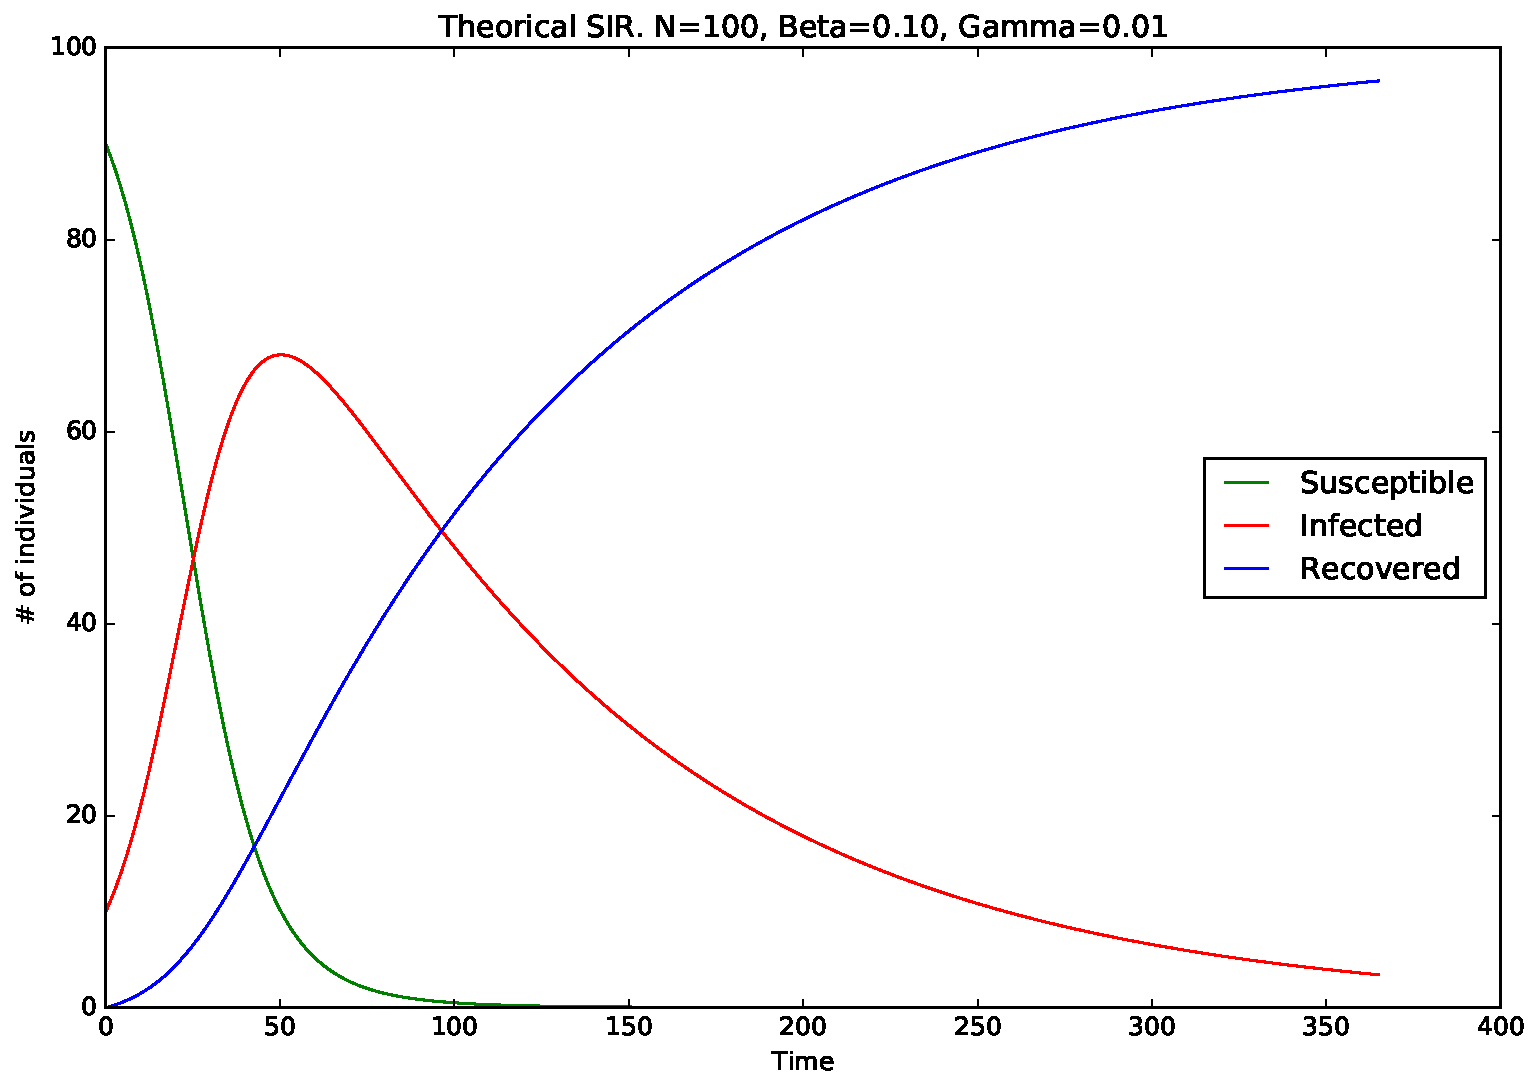
\includegraphics[width= 1.0 \linewidth]{plots/sir_one_region.pdf}
	\caption{Numerical solution to the nonlinear ODE system defining the SIR model.}
\end{figure}




\subsection{Multi-compartment SIR}